Im Versuch werden die Übergänge des Cadmiums unter Aufspaltung durch den Zeeman-Effekt betrachtet.
Dem roten Licht liegt dabei der normale Zeeman-Effekt zugrunde, dem blauen Licht der anormale Zeeman-Effekt.\\
Der Landé-Faktor des Übergangs $g_{12}$ ergibt sich für den normalen Zeeman-Effekt (rot) zu
\begin{equation*}
  g_{ij}  &= \SI{0.974 \pm 0.011}{}.
\end{equation*}
was mit einer relativen Abweichung von $f=\SI{2.65}{\%}$ zum theoretischen Landé-Faktor
\begin{equation*}
  g_{12, \text{theo}} = \SI{1}{}
\end{equation*}
des zirkularen Übergangs passt.
\begin{figure}[h!]
  \centering
  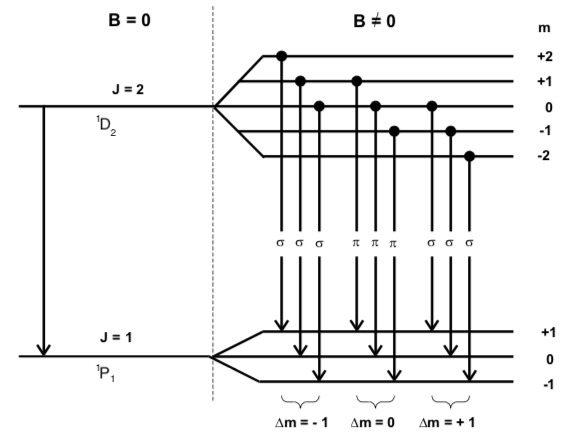
\includegraphics[width=\textwidth]{normal.png}
  \caption{Aufspaltung durch den normalen Zeeman-Effekt \cite{1}}
  \label{fig:normal}
\end{figure}
\FloatBarrier
Für die Übergänge des anormalen Zeeman-Effekts werden die Landé-Faktoren des Übergangs $g_{ij}=m_{1}g_{1}-m_{2}g_{2}$ berechnet und mit der Theorie verglichen.
Der theoretische Wert für $\sigma$ mittelt sich hier aus den Werten $g_{12, \text{theo}, 1}=2$ und $g_{12, \text{theo}, 2}=\frac{3}{2}$, da sich die Linien durch den optischen Doppler-Effekt stark überlagern, die Messung aber über die Mitte der Linie ausgeführt wird.
Wiederum der zweite theoretische Wert für den $\pi$-Übergang $g_{12, \text{theo}} = 0 $ ist stark unterdrückt und fällt im Mittel nicht ins Gewicht.
So ergibt sich:
\begin{align*}
  \sigma  &&& g_{12, \text{exp}} &= \SI{1.30 \pm 0.02}{}    &&&   g_{12, \text{theo}} &= \SI{1.75}{}     &&&  f=\SI{25.71}{\%}   \\
  \pi     &&& g_{12, \text{exp}} &= \SI{0.442 \pm 0.004}{}  &&&   g_{12, \text{theo}} &= \SI{0.5}{}   &&&  f=\SI{11.60}{\%}   .
\end{align*}
\begin{figure}[h!]
  \centering
  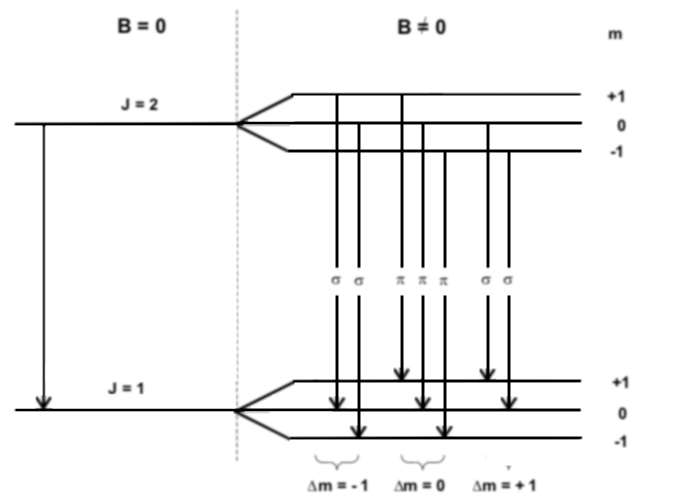
\includegraphics[width=\textwidth]{anormal.png}
  \caption{Aufspaltung durch den anormalen Zeeman-Effekt \cite{1}}
  \label{fig:normal}
\end{figure}
\FloatBarrier
Mögliche Erklärungen für die Abweichungen sind der bereits genannte optische Doppler-Effekt, 
